% !TEX root = ../my-thesis.tex
%
\chapter{Surrogate-Based Accelerated Calibration}
\label{sec:surr}

\cleanchapterquote{Per correr miglior acque alza le vele; omai la navicella del mio ingegno ...}{Dante Alighieri (Divina Commedia)}{Italian Poet (1265-1321)}

\section{Introduction}
\label{sec:surr:intro}

In the previous chapter we presented the \gls{cmp} method, which consists of a modular approach to perform the Bayesian calibration of a computer code. The \gls{cmp} method splits the calibration process into two steps: the estimation of the model error hyperparameters, $\psimap$, and the evaluation of the posterior distribution of the parameters, $\p{\btheta \mid \data}$. The key advantage of the \gls{cmp} method is that it provides a better approximation of the posterior distribution of the parameters, $\btheta$, by allowing the model error hyperparameters, $\bpsi$, to depend on the parameters, $\btheta$. However, this flexibility comes at a cost since estimating $\psimap$ requires solving an optimization problem at each sample, which can be computationally expensive. 

\smallskip
In this chapter we propose to alleviate the computational cost of the \gls{cmp} method by relaxing the definition of $\psimap$, replacing expensive queries to the optimizer with cheap queries to a surrogate model. To lay the groundwork for this chapter, let us first rewrite the \gls{cmp} distribution, Eq.~\eqref{eq:cmp:cmp}, in the following way,

\begin{equation}
  \begin{aligned}
    \mathrm{p}(\btheta \mid \data) &\appropto \prior{\btheta} \, \exp\left(-\phi(\btheta \mid \psimap)\right)\;, \\
    \text{with } \phi(\btheta \mid \psimap) &= -\log \likelihood{\data \mid \btheta, \psimap} - \log \prior{\psimap} + \log \detf{\Stheta}\;.
  \end{aligned}
  \label{eq:surr:cmp}
\end{equation}

Eq.~\eqref{eq:surr:cmp} highlights the fact that the \gls{cmp} method can be interpreted as a potential-based method, where the potential, $\phi(\btheta \mid \psimap)$, is a function of the hyperparameters, $\psimap$. The potential is defined as the negative log of the unnormalized posterior distribution, which is the product of the likelihood and the prior distribution of the parameters, $\btheta$, and the hyperparameters, $\bpsi$. The correction term, $\log \detf{\Stheta}$, is needed to preserve the structure of the posterior distribution when $\psimap$ depends on $\btheta$. This term is defined as the determinant of a Hessian matrix and can be interpreted as a correction factor that accounts for the change in volume of the parameter space induced by the dependence of $\psimap$ on $\btheta$.

\smallskip
The surrogate-strategy proposes to replace $\psimap$ with a surrogate model, $\tilde{\bpsi}(\btheta)$. The literature offers many non-intrusive techniques to build surrogate models, but in this chapter we focus on \glspl{gp} for their flexibility and their ability to (cheaply) provide accurate uncertainty estimates, which, as we will see, will become very useful for the techniques developed in the remainder of this chapter. The computational cost for querying a \gls{gp} model is proportional to the size of the training set $\ntrain$ for the predictive mean and proportional to $\ntrain^2$ for the predictive variance. Furthermore, selecting the hyperparameters for the \gls{gp} can be computationally expensive as it depends on the cube of the training set size, $\ntrain^3$. Keeping the size of the training set small is therefore critical to keep the cost contained. Unfortunately, the accuracy of the surrogate model also increases with the size of the training set, which creates a clear trade-off between the cost and the accuracy of the surrogate model. The exact dependence between the size of the training set and the accuracy of the surrogate model is problem dependent and depends on the complexity of the function being approximated. In the context of \glspl{gp}, the complexity of the function is often related to the lengthscale of the covariance function, with shorter lengthscales corresponding to more complex functions. In general, more complex functions require larger training sets to be accurately approximated. 

\smallskip
On the other hand, the size of the training set is not the only free parameter that can be tuned, as one also needs to choose the locations of the training points. This problem is known as the \gls{doe} and is a well-studied problem in the literature. To further motivate the importance of the \gls{doe}, let us consider the expected error between the true potential $\phi(\btheta \mid \psimap)$ and the surrogate potential $\phi(\btheta \mid \tilde{\bpsi}(\btheta))$,

\begin{equation}
  \mathcal{E} = \int_{\Theta}  \left(\phi(\btheta \mid \psimap) - \phi(\btheta \mid \tilde{\bpsi}(\btheta)) \right)^2  \,\mathbb{P}(\dd \btheta)\;,
\end{equation}

where $\mathbb{P}(\dd \btheta)$ is a probability measure over the parameter space, $\Theta$. The question now is \textit{What is the most appropriate measure?} A first choice could be a uniform measure over the parameter space, i.e. $\mathbb{P}(\dd \btheta) \propto 1$, which corresponds to a traditional space-filling one-shot design, such as \gls{lhs}~\cite{Dutta2019}. Other popular choices include the prior distribution of the parameters, $\prior{\btheta}$~\cite{marzouk2007, marzouk2009}. However, both of these choices are not ideal since the prior distribution is often very broad and the posterior distribution is often concentrated in small regions of the parameter space, especially for high-dimensional problems. A more appropriate choice would be the posterior distribution of the parameters, $\p{\btheta \mid \data}$, since it is the distribution of interest and is often concentrated in small regions of the parameter space. Unfortunately, the posterior distribution is unknown a priori, which creates a chicken-and-egg problem since we need to build an accurate surrogate model to estimate the posterior distribution, but we also need the posterior distribution to build an accurate surrogate model. The work of~\cite{lucor2018} was one of the first to propose a solution to this problem by introducing an iterative algorithm. The algorithm starts with an initial surrogate model built with a traditional one-shot design, such as \gls{lhs}, and then iteratively enriches the training set with new points sampled from the current estimate of the posterior distribution. This strategy is referred to as an \gls{as} strategy. It is particularly beneficial in high-dimensional parameter spaces, a capability that will be explicitly demonstrated in Chapter~\ref{sec:cfd}, and can significantly reduce the size of the training set needed to achieve a given accuracy compared to traditional one-shot designs, here denoted as \gls{lhs} strategies. The main drawback of \gls{as} strategies is that they introduce an offline overhead to build the surrogate model, which can be significant if the number of iterations required is large or if the cost of building the surrogate model is high. However, this offline cost can be justified if the online cost of querying the surrogate model is significantly lower than the cost of solving the optimization problem at each sample.

\smallskip
Before delving into the details of the surrogate-based speed-up strategy, we need to discuss another important detail. Specifically, we stated that the surrogate model is used to replace $\psimap$ in the potential, $\phi(\btheta \mid \psimap)$, but why not replace the entire potential with a surrogate model, $\tilde{\phi}(\btheta)$? We refer to such a strategy as the \gls{lpgp} method, since the surrogate model is built for the log-posterior distribution of the parameters and to the first strategy as the hyperparameter \gls{hgp} method, since the surrogate model is built for the hyperparameters. 

\smallskip
The \gls{lpgp} method would further reduce both the offline and online costs since it would also replace the likelihood evaluation with a surrogate model, and require a single surrogate model to be built, instead of one surrogate model per hyperparameter. On the other hand, the \gls{hgp} strategy has the advantage of preserving the structure of the posterior distribution, which improves the accuracy. This is because the likelihood is a function of the hyperparameters, $\psimap$, and the residuals between the model and the data, which are critical to capture the structure of the posterior distribution. When the residuals are high, the likelihood is low and, even if the surrogate model for the hyperparameters is not very accurate, the posterior distribution will be low in those regions of the parameter space. The \gls{lpgp} method, on the other hand, is unaware of this structure since it replaces the entire potential with a surrogate model, and therefore may require a larger training set to globally explore the whole parameter space and capture the structure of the posterior distribution, which can be very challenging for high-dimensional problems. Furthermore, the \gls{hgp} method provides direct access to the hyperparameters, $\psimap$, which are needed to compute the predictive distribution and to evaluate the model error, while the \gls{lpgp} method does not provide direct access to these hyperparameters since they are implicitly included in the surrogate model for the potential.

\smallskip
In \S\ref{sec:surr:perf-cmp-calbr} we first formalize these ideas by discussing the computational cost of the \gls{cmp} method and of the surrogate-based speed-up strategy, i.e.,

\begin{enumerate}
  \item \gls{lhs}-\gls{hgp}: surrogate model for the hyperparameters built with a traditional one-shot design, such as \gls{lhs}.
  \item \gls{as}-\gls{hgp}: surrogate model for the hyperparameters built with an \gls{as} strategy.
  \item \gls{lhs}-\gls{lpgp}: surrogate model for the potential built with a traditional one-shot design, such as \gls{lhs}.
  \item \gls{as}-\gls{lpgp}: surrogate model for the potential built with an \gls{as} strategy.
\end{enumerate}

In \S\ref{sc:surr:accel-calibr} we present the surrogate-based speed-up strategy to accelerate the \gls{cmp} calibration process, which consists in building a surrogate model for the hyperparameters, $\psimap$, using an \gls{as} strategy. The technical details are developed for the \gls{hgp} method, but they can be easily adapted to the \gls{lpgp} method as well, as briefly discussed in \S\ref{sc:surr:lpgp}. Finally, in \S\ref{sc:surr:examples} we present some numerical results to compare the different methods and to show the benefits of the surrogate-based speed-up strategy.

\smallskip
This chapter is based on a contribution published in the \textit{Journal of Mechanical Design}~\cite{surr} in which we present the surrogate-based speed-up strategy to accelerate the \gls{cmp} calibration process. 

\section{Cost Analysis of the CMP Method}
\label{sec:surr:perf-cmp-calbr}

In this subsection we discuss the computational cost of the \gls{cmp} method and show how introducing a surrogate model for $\psimap$ can alleviate such cost. Evaluating the \gls{cmp} distribution, Eq.~\eqref{eq:cmp:cmp}, or the predictive distribution, Eq.~\eqref{eq:cmp:pred}, requires two expensive steps:

\begin{enumerate}
  \item Evaluating the forward model, $f(\bx; \btheta)$.
  \item Solving the optimization problem of Eq.~\eqref{eq:cmp:hp_cmp} to estimate the hyperparameters, $\psimap$.
\end{enumerate}

Evaluating the forward model is often the most expensive part of the calibration process. In engineering applications, this cost is due to the complexity of the model and is usually dominant. To alleviate this problem, practitioners often replace calls to the forward model with calls to a cheaper surrogate model, $f(\bx; \btheta) \rightarrow \tilde{f}(\bx; \btheta)$. Given this need, one could suggest to build $\tilde{f}(\bx, \btheta)$ online to minimize the difference with $f$ under the posterior distribution of the parameters, $\p{\btheta \mid \data}$. Although appealing in theory, this strategy is not ideal in practice. First and foremost, building the surrogate model online requires evaluating the true forward model during the iterative loop. In some engineering pipelines, this could be problematic since the forward can't be evaluated interactively at the required cadence or on the same hardware used for the calibration process. Most importantly, we might need to inspect several different posteriors (different datasets, different priors, etc.) and building a surrogate model for each of them would be infeasible. Finally, calibration is only one use-case: the surrogate is often needed for other tasks such as sensitivity analysis or real-time control. 

\smallskip
Given the above reasons, treating $f(\bx;\btheta)$ as an extra hyperparameter and building it along with $\tilde{\psi}(\btheta)$ does not seem to be a good idea, and we prefer to separate the construction of the surrogate model for the forward model from the construction of the surrogate model for the hyperparameters. Finally, when $\tilde{f}(\bx; \btheta)$ is not precise enough (for example because it was built using a small and non-adaptive training set), the effect of this error on the calibration process is to introduce an extra source of model error. This extra source of error is to be intended as a \textit{discretization error} and would be captured in the estimation of $z(\bx; \bpsi)$, which is the model error term in the \gls{cmp} method. We prefer therefore to focus our efforts on accelerating the \gls{cmp} method by building a surrogate model for the hyperparameters, $\psimap$, while treating the surrogate model for the forward model as a separate problem.

\smallskip
Concerning the \gls{cmp} method, estimating $\psimap$ through Eq.~\eqref{eq:cmp:hp_cmp} is the most expensive step since it scales as the number of hyperparameters, $\nhyper$, and the cost of inverting the likelihood, for which a Cholesky decomposition is often used. The cost of the Cholesky decomposition scales as $\mathcal{O}(\nobs^3)$. Therefore, the overall cost of estimating $\psimap$ scales as $\mathcal{O}(\nhyper \, \nobs^3)$. Furthermore, multiple evaluations of the likelihood and its gradients are required to solve the optimization problem, increasing the overall cost.

\smallskip
To reduce the cost of estimating $\psimap$, we propose to use a surrogate model for the hyperparameters, here denoted explicitly as $\tilde{\bpsi}(\btheta)$, which can be evaluated at a negligible cost compared to the optimization problem of Eq.~\eqref{eq:cmp:hp_cmp}. If multi-output \glspl{gp} are used, the cost would be proportional to $\mathcal{O}(\nhyper \, \ntrain)$, with $\ntrain$ the number of training points used to build the surrogate model. As said before, this strategy is referred to as the \gls{hgp} strategy and is combined with either a \gls{lhs} sampling or an \gls{as} strategy to efficiently build the training set. For the first, the offline building cost of the \glspl{hgp} scales as $\mathcal{O}(\nhyper \, \ntrain^3)$, while for the second it scales as $\mathcal{O}({\niter} \, \nhyper \, \ntrain^3)$, with ${\niter}$ the number of iterations required by the adaptive strategy. 

\smallskip
In contrast, the \gls{lpgp} strategy builds a surrogate model for the potential, $\phi(\btheta \mid \psimap)$, which is a scalar quantity. Therefore, both offline and online costs are significantly reduced since only a single surrogate model needs to be built and queried.

\smallskip
A question that naturally arises is how the \gls{hgp} and \gls{lpgp} methods treat the correction term, $\log \detf{\Stheta}$, function of $\psimap$. In the \gls{lpgp} method, this term is not explicitly reconstructed but is implicitly included in the surrogate model for the potential. In the \gls{hgp} method, this term can be evaluated using the surrogate model for $\psimap$. However, $\log \detf{\Stheta}$ is defined as the determinant of a Hessian matrix, a quantity well-defined only for negative definite matrices. If the \glspl{hgp} are not accurate enough, the correction term may become undefined, or may bring huge errors. To avoid this problem, we propose to treat the correction term as an extra hyperparameter and build a surrogate model for it as well. In the remainder of this chapter, the quantity $\tilde{\bpsi}(.)$ will be used to denote the surrogate model for the hyperparameters, $\psimap$, and the correction term, $\log \detf{\Stheta}$.

\begin{table}[htbp]
  \centering
  \small
  \begin{tabular}{|l|c|c|c|c|}
    \hline
    \textbf{Method} 
    & \multicolumn{1}{c|}{\textbf{Offline overhead}} 
    & \multicolumn{2}{c|}{\textbf{Online overhead (per sample)}}
    & \textbf{Accuracy} \\
    \cline{2-4}
    & build/training 
    & query 
    & likelihood 
    &  \\
    \hline
    \gls{cmp}
    & -- 
    & $\mathcal{O}(\nhyper\,\nobs^3)$ 
    & $\mathcal{O}(\nobs^3)$
    & Exact \\
    \hline
    \gls{as}-\gls{hgp} 
    & $\mathcal{O}({\niter} \, \nhyper \, \ntrain^3)$ 
    & $\mathcal{O}(\nhyper\,\ntrain)$ 
    & $\mathcal{O}(\nobs^3)$
    & Very High \\
    \hline
    \gls{lhs}-\gls{hgp} 
    & $\mathcal{O}(\nhyper \, \ntrain^3)$ 
    & $\mathcal{O}(\nhyper\,\ntrain)$ 
    & $\mathcal{O}(\nobs^3)$
    & Low \\
    \hline
    \gls{as}-\gls{lpgp} 
    & $\mathcal{O}({\niter} \, \ntrain^3)$ 
    & -- 
    & $\mathcal{O}(\ntrain)$ (no likelihood)
    & High \\
    \hline
    \gls{lhs}-\gls{lpgp} 
    & $\mathcal{O}(\ntrain^3)$ 
    & -- 
    & $\mathcal{O}(\ntrain)$ (no likelihood)
    & Very Low \\
    \hline
  \end{tabular}
  \caption{Summary of the computational costs of the different methods. $\nobs$ is the number of observations, $\nhyper$ the number of hyperparameters, $\ntrain$ the number of training points used to build the surrogate model, ${\niter}$ the number of iterations required by the adaptive strategy.}
  \label{tab:method_costs_small}
\end{table}


Tab.~\ref{tab:method_costs_small} summarizes the computational costs of the different methods discussed above. The \gls{cmp} method is the most expensive since it requires solving an optimization problem at each sample. The \gls{hgp} methods reduce this cost by introducing a surrogate model for the hyperparameters, while the \gls{lpgp} methods further reduce the cost by avoiding the likelihood evaluation. \gls{as} strategies introduce an offline overhead to build a more accurate surrogate model, while \gls{lhs} strategies have a lower offline cost but may require a larger training set to achieve the same accuracy. The choice between these methods is a clear trade-off between offline and online costs, as well as the desired accuracy and availability of hyperparameters.

\smallskip
We can however expect \gls{hgp} methods to be more accurate than \gls{lpgp} methods since they preserve the structure of the posterior distribution and provide direct access to the hyperparameters. Furthermore, since \gls{as} strategies build a training set in regions of the parameter space that are more likely a posteriori, we can expect them to be more accurate than \gls{lhs} strategies for a given training set size. The goal is therefore to build an accurate surrogate model of $\psimap$ with a limited number of training points, $\ntrain$, and a limited number of iterations, ${\niter}$, to keep both offline and online costs low. In the following section we present such a strategy.

\section{Methodology: Accelerated CMP Via Surrogate Modeling}
\label{sc:surr:accel-calibr}

In this section we discuss the surrogate-based speed-up strategy to accelerate the \gls{cmp} calibration process. In \S\ref{sc:surr:surrogate} we introduce a surrogate model for the model error hyperparameters, $\psimap$, and in \S\ref{sc:surr:iterative} we present an iterative algorithm to build the surrogate model.

\subsection{Hyperparameter Gaussian Processes}
\label{sc:surr:surrogate}

In this section we discuss some technical details regarding the construction of the \glspl{hgp} used to approximate $\psimap$. Recall from \S\ref{sec:sota_1} the hyperparameters space $\Psi \subset \reals^{\nhyper}$, with $\nhyper$ being the number of hyperparameters (including the correction factor $\detf{\Stheta}$). Secondly, let's introduce the training set $\boldsymbol{\Psi} = \{\bpsi(\btheta_i)\}_{i=1}^{\ntrain}$ where $\bpsi(\btheta_i)$ denotes the vector containing the \gls{cmp} definition of the hyperparameters $\psimap$ and the correction factor $\detf{\Stheta}$. We wish to build a \gls{gp} to interpolate the training data.

\smallskip
Since the function $\bpsi(\btheta)$ is multi-output, we can't use directly the techniques discussed in \S\ref{sec:ntools:gpr} but resort to a technique introduced by~\cite{wilkinson2010}. Specifically, each component of $\bpsi(\btheta)$ will be modeled as a linear combination of $\tilde{N}_{\mathrm{hyper}}$ scalar independent \glspl{gp}, here denoted by $h_i(\btheta) \sim \mathcal{\gls{gp}}(m_{\boldsymbol{\beta}_i}(\cdot), k_{\boldsymbol{\beta}_i}(\cdot, \cdot))$, with $\boldsymbol{\beta}_i$ denoting the hyperparameters that parameterize the mean and covariance functions of each \gls{gp}. As we'll see, the number of independent \glspl{gp}, $\tilde{N}_{\mathrm{hyper}}$, can be less than the actual number of \glspl{hgp} $\nhyper$. We note this linear combination with,

\begin{equation}
  \tilde{\bpsi}(\btheta) = \boldsymbol{\mu} + \mathbf{W} \begin{bmatrix} h_1(\btheta) \\ \vdots \\ h_{\tilde{N}_{\mathrm{hyper}}}(\btheta) \end{bmatrix} \;.
  \label{eq:multiout}
\end{equation}

With $\boldsymbol{\mu} \in \reals^{\nhyper}$ and $\mathbf{W} \in \reals^{\nhyper \times \tilde{N}_{\mathrm{hyper}}}$ two constant matrices. To compute those matrices we perform a \gls{pca} on the training set $\boldsymbol{\Psi}$. 

\smallskip
Specifically, the mean vector is computed as:
\begin{equation}
  \boldsymbol{\mu} = \frac{1}{\ntrain} \displaystyle\sum_{i=1}^{\ntrain} \bpsi(\btheta_i) \;.
  \label{eq:pca_mean}
\end{equation}

The centered data matrix $\mathbf{X}_c \in \reals^{\ntrain \times \nhyper}$ is constructed by subtracting the mean from each training point:
\begin{equation}
  \mathbf{X}_c = \begin{bmatrix} \bpsi(\btheta_1) - \boldsymbol{\mu} \\ \vdots \\ \bpsi(\btheta_{\ntrain}) - \boldsymbol{\mu} \end{bmatrix}^{\top} \;.
  \label{eq:pca_centered}
\end{equation}

The covariance matrix is then given by:
\begin{equation}
  \boldsymbol{\Sigma} = \frac{1}{\ntrain - 1} \mathbf{X}_c^{\top} \mathbf{X}_c \;,
  \label{eq:pca_cov}
\end{equation}

whose eigendecomposition yields eigenvectors $\mathbf{v}_j$ and eigenvalues $\lambda_j$ ordered in descending order: $\lambda_1 \geq \lambda_2 \geq \cdots \geq \lambda_{\nhyper}$. We select the first $\tilde{N}_{\mathrm{hyper}}$ eigenvectors corresponding to the largest eigenvalues, and construct the matrix $\mathbf{W}$ as:
\begin{equation}
  \mathbf{W} = \begin{bmatrix} \sqrt{\lambda_1} \mathbf{v}_1 & \sqrt{\lambda_2} \mathbf{v}_2 & \cdots & \sqrt{\lambda_{\tilde{N}_{\mathrm{hyper}}}} \mathbf{v}_{\tilde{N}_{\mathrm{hyper}}} \end{bmatrix} \;.
  \label{eq:pca_loadings}
\end{equation}

This approach is beneficial when the hyperparameters exhibit strong correlations or when some dimensions contribute negligibly to the overall variability, as it reduces the number of independent \glspl{gp} needed while preserving the essential structure of the hyperparameter space. The number $\tilde{N}_{\mathrm{hyper}}$ is typically chosen to explain a target fraction (e.g., 95\%) of the total variance: $\sum_{j=1}^{\tilde{N}_{\mathrm{hyper}}} \lambda_j / \sum_{j=1}^{\nhyper} \lambda_j \geq 0.95$. Furthermore, each \gls{gp} $h_i(\btheta)$ is trained independently using the corresponding column of $\mathbf{W}$ as the target values for the training set, i.e. $h_i(\btheta) \sim \mathcal{\gls{gp}}(m_{\boldsymbol{\beta}_i}(\cdot), k_{\boldsymbol{\beta}_i}(\cdot, \cdot) \mid \mathbf{W}_{:, i})$, where $\mathbf{W}_{:, i}$ denotes the $i$-th column of $\mathbf{W}$. The hyperparameters $\boldsymbol{\beta}_i$ of each \gls{gp} are estimated using the training set and can be optimized using techniques such as \gls{mle} or \gls{map} estimation. 

\smallskip
The mean and covariance functions of the resulting multi-output \gls{gp}, $\tilde{\bpsi}(\btheta)$, can be derived from the mean and covariance functions of the independent \glspl{gp}, $h_i(\btheta)$. Specifically, the mean function of $\tilde{\bpsi}(\btheta)$ is given by:

\begin{equation}
  \mathbf{m}_{\tilde{\bpsi}}(\btheta) = \boldsymbol{\mu} + \mathbf{W} \begin{bmatrix} m_{\boldsymbol{\beta}_1}(\btheta) \\ \vdots \\ m_{\boldsymbol{\beta}_{\tilde{N}_{\mathrm{hyper}}}}(\btheta) \end{bmatrix} \;,
  \label{eq:multiout_mean}
\end{equation}
and the covariance function is given by:

\begin{equation}
  \mathbf{K}_{\tilde{\bpsi}}(\btheta, \btheta') = \mathbf{W} \begin{bmatrix} k_{\boldsymbol{\beta}_1}(\btheta, \btheta') & 0 & \cdots & 0 \\ 0 & k_{\boldsymbol{\beta}_2}(\btheta, \btheta') & \cdots & 0 \\ \vdots & \vdots & \ddots & \vdots \\ 0 & 0 & \cdots & k_{\boldsymbol{\beta}_{\tilde{N}_{\mathrm{hyper}}}}(\btheta, \btheta') \end{bmatrix} \mathbf{W}^{\top} \;.
  \label{eq:multiout_cov}
\end{equation}

\smallskip
Finally, since the \glspl{hgp} are random functions, the surrogate model for the hyperparameters, $\tilde{\bpsi}(\btheta)$, is also a random function. A realization of this function $\tilde{\bpsi}^{(\boldsymbol{\omega})}(\btheta)$ can be obtained by sampling a trajectory of each \gls{gp}, $h_i^{(\omega_i)}(\btheta)$, and then applying the linear transformation defined in Eq.~\eqref{eq:multiout}. Here $\boldsymbol{\omega} = (\omega_1, \ldots, \omega_{\tilde{N}_{\mathrm{hyper}}})$ is a vector of random variables that parameterize the trajectories of the \glspl{gp}. The distribution of $\tilde{\bpsi}(\btheta)$ is therefore defined by the distribution of the \glspl{gp} and the linear transformation. The corresponding estimate of the posterior distribution of the parameters, $\btheta$, given a realization of the surrogate model for the hyperparameters, $\tilde{\bpsi}^{(\boldsymbol{\omega})}(\btheta)$, can be obtained by replacing $\psimap$ with $\tilde{\bpsi}^{(\boldsymbol{\omega})}(\btheta)$ in the potential, $\phi(\btheta \mid \psimap)$,

\begin{equation}
  \p{\btheta \mid \data, \boldsymbol{\omega}} = \prior{\btheta} \ \dfrac{\exp \left(-\phi(\btheta \mid \tilde{\bpsi}^{(\boldsymbol{\omega})}(\btheta)) \right)}{\gamma(\boldsymbol{\omega})} \;.
  \label{eq:phik}
\end{equation}

The random variable $\gamma(\boldsymbol{\omega})$ ensures that the distribution is normalized.

\subsection{Adaptive Sampling Strategy AS-HGP}
\label{sc:surr:iterative}

The construction of the surrogate model for the hyperparameters, $\tilde{\bpsi}(\btheta)$, requires the selection of the training set, $\boldsymbol{\Psi}$. As discussed in \S\ref{sec:surr:intro}, the choice of the training set is critical to achieve a good accuracy with a limited number of training points, $\ntrain$. Traditional one-shot designs, such as \gls{lhs}, build the training set without any knowledge of the posterior distribution, which can lead to a poor accuracy if the posterior distribution is concentrated in small regions of the parameter space. On the other hand, \gls{as} strategies build the training set in regions of the parameter space that are more likely a posteriori, which can significantly improve the accuracy for a given training set size.

\smallskip
Since the posterior distribution is unknown a priori, we need to use an iterative algorithm to build the training set. The algorithm starts with an initial training set, $\boldsymbol{\Psi}^{(0)}$, which can be built using a traditional one-shot design, such as \gls{lhs}. At each iteration $k$, the algorithm enriches the training set by adding new points from the current estimate of the posterior distribution, $\mathrm{p}^{(k)}(\btheta \mid \data)$. 

\begin{algorithm}[htbp]
    \small % Change font size here
    \begin{algorithmic}[1]
      \Require An initial training set, $\boldsymbol{\Psi}^{(0)}$.
      \Ensure A surrogate model of the model error, $\tilde{\boldsymbol{\psi}}^{(\star)}(\boldsymbol{\theta})$.
  
      \While{Not converged.}
        \State Build $\tilde{\boldsymbol{\psi}}^{(k)}(\boldsymbol{\theta})$ using the training set, $\boldsymbol{\Psi}^{(k)}$ as described in \S\ref{sc:surr:surrogate}.
        \State Sample a candidate set of points from the current estimate of the posterior distribution, $\boldsymbol{\Theta}_c^{(k)} = \{\boldsymbol{\theta}^i\}_{i=1}^{\ncand} : \boldsymbol{\theta}_i \sim \mathrm{p}^{(k)}(\boldsymbol{\theta} \mid \data)$ (Section \ref{sc:surr:candidate}).
        \State Resample the candidate set to select ${\nresample}$ new training points (weighted resampling). Create the resampled set, $\boldsymbol{\Theta}_r^{(k)} = \{\boldsymbol{\theta}^i\}_{i=1}^{\nresample} : \boldsymbol{\theta}_i \in \boldsymbol{\Theta}_c^{(k)}$ (Section \ref{sc:surr:select}).
        \State Update the training set, $\boldsymbol{\Psi}^{(k+1)} = \boldsymbol{\Psi}^{(k)} \cup \{\boldsymbol{\psi}(\boldsymbol{\theta}_i)\}_{i=1}^{\nresample} : \boldsymbol{\theta}_i \in \boldsymbol{\Theta}_r^{(k)}$.
      \EndWhile
    \end{algorithmic}
    \caption{Adaptive construction of the surrogate of the model error.}
    \label{alg:adapt_surr}
\end{algorithm}

The algorithm in \ref{alg:adapt_surr} describes the iterative construction of the surrogate model of the model error, $\tilde{\boldsymbol{\psi}}(\boldsymbol{\theta})$. The algorithm starts with an initial training set, $\boldsymbol{\Psi}^{(0)}$, and iteratively enriches it, at each step $k$, by adding new points from the current estimate of the posterior distribution, $\mathrm{p}^{(k)}(\boldsymbol{\theta} \mid \data)$. The algorithm stops when a stopping criterion is met, which can be a fixed number of iterations or a convergence criterion.

\smallskip
The first step of the algorithm is to build the surrogate model for the hyperparameters, $\tilde{\boldsymbol{\psi}}^{(k)}(\boldsymbol{\theta})$, using the current training set, $\boldsymbol{\Psi}^{(k)}$, as described in \S\ref{sc:surr:surrogate}. The second step is to sample a candidate set of points from the current estimate of the posterior distribution, $\mathrm{p}^{(k)}(\boldsymbol{\theta} \mid \data)$, which is discussed in \S\ref{sc:surr:candidate}. The third step is to resample the candidate set to select ${\nresample}$ new training points, which are added to the training set for the next iteration. The resampling strategy is discussed in more detail in \S\ref{sc:surr:select}.

\subsubsection{Posterior-Informed Candidate Sampling}
\label{sc:surr:candidate}

A key step of the algorithm is the construction of the candidate set, $\boldsymbol{\Theta}_c^{(k)}$, which is used to select the points to be added to the training set. The candidate set is built by sampling $\ncand$ points from the current estimate of the posterior distribution, $\mathrm{p}^{(k)}(\boldsymbol{\theta} \mid \data)$. This distribution was not defined yet, but it can be obtained by averaging the distribution in Eq.~\eqref{eq:phik} over different realizations of the \glspl{hgp},

\begin{equation}
  \left.
    \begin{aligned}
      \mathrm{p}^{(k)}(\boldsymbol{\theta} \mid \data) &= \mathbb{E}_{\boldsymbol{\omega}} \left[\mathrm{p}^{(k)}(\boldsymbol{\theta} \mid \data, \boldsymbol{\omega})\right]\\
      &=\prior{\boldsymbol{\theta}} \ \mathbb{E}_{\boldsymbol{\omega}} \left[ \dfrac{\exp \left(-\phi(\boldsymbol{\theta} \mid \tilde{\boldsymbol{\psi}}^{(\boldsymbol{\omega})}(\boldsymbol{\theta}; \boldsymbol{\beta}^{(k)})) \right)}{\gamma(\boldsymbol{\omega})} \right]\;.
    \end{aligned}
  \right.
    \label{eq:avg_dist}
\end{equation}

Note that we have changed the notation of the surrogate model $\tilde{\boldsymbol{\psi}}(\boldsymbol{\theta})$ to $\tilde{\boldsymbol{\psi}}^{(\boldsymbol{\omega})}(\boldsymbol{\theta}; \boldsymbol{\beta}^{(k)})$ to explicitly indicate that it is a random function defined by the hyperparameters of the \glspl{gp}, $\boldsymbol{\beta}^{(k)}$, and the random variables that parameterize the trajectories of the \glspl{gp}, $\boldsymbol{\omega}$. 

\smallskip
Unfortunately, the expectation in Eq.~\eqref{eq:avg_dist} is intractable, especially because the normalization factor $\gamma(\boldsymbol{\omega})$ is unknown. To estimate it efficiently, we use a \gls{mc} approach and sample $\ncand/M$ points from $M$ different realizations of the current estimate of the posterior distribution, $\mathrm{p}^{(k)}(\boldsymbol{\theta} \mid \data, \boldsymbol{\omega}_i),\; i=1\ldots M$. Each realization is obtained from a different random trajectory of the \glspl{hgp}, $\tilde{\boldsymbol{\psi}}^{(\boldsymbol{\omega})}(\boldsymbol{\theta}; \boldsymbol{\beta}^{(k)})$. As a rule of thumb, we use $M=20$ realizations, which is often enough to obtain a good approximation of the averaged posterior distribution. 

\smallskip
In practice, the candidate set is built by sampling different \gls{mcmc} chains, a process that can be easily parallelized, and then merging the samples. To parametrically evaluate a random realization of a \gls{gp} we use the technique discussed in \S\ref{sec:ntools:gpr}.

\smallskip
A question that naturally arises is \textit{Why don't we simply use the predictive mean of the surrogate model for the hyperparameters, $\mathbf{m}_{\tilde{\bpsi}}(\btheta \mid \boldsymbol{\Psi})$, to build the candidate set?} The reason is overfitting. Indeed, the predictive mean of the surrogate model is a good approximation of the true $\psimap$ in regions of the parameter space that are close to the training points, but it can be a poor approximation in regions that are far from the training points. At later iterations, when the training set is rich enough, using the predictive mean is a good strategy to build the candidate set, but at early iterations it can lead to a biased estimation of the candidate set. This is because the candidate set is drawn from the current estimate of the posterior distribution, which is defined by the surrogate model for the hyperparameters. If the surrogate model is not accurate enough, the candidate set will be drawn from a biased distribution, which can lead to a poor selection of the training points and slow down the convergence of the algorithm. By sampling different trajectories of the hyperparameters we can mitigate this problem and obtain a candidate set that is more representative of the global uncertainty.

\subsubsection{Variance-Based Weighted Resampling}
\label{sc:surr:select}

In this section we discuss a weighted resampling strategy to select ${\nresample}$ points from the candidate set, $\boldsymbol{\Theta}_c^{(k)}$, to be added to the training set. The goal of this step is to select points which would substantially improve the surrogate model. In order to do so, we propose to use a resampling strategy inspired by~\cite{gelman2014} and use as resampling weight, $w_{\mathrm{res}}(\btheta_i)$, the variance of the potential,

\begin{equation}
  w_{\mathrm{res}}(\btheta_i) \propto \mathbb{V}_{\boldsymbol{\omega}} \left[ \phi(\btheta_i \mid \tilde{\bpsi}^{(\boldsymbol{\omega})}(\btheta_i))\right] \;.
  \label{eq:var}
\end{equation}

Intuitively, points with high variance come from regions of the support in which the model error is less known and affects the potential the most. The resulting strategy is therefore a good balance between exploitation and exploration of the parameter space.
The variance of the potential can be cheaply estimated using a first order Taylor expansion,

\begin{equation}
  \left. 
      \begin{aligned}
        \mathbb{V}_{\boldsymbol{\omega}} \left[ \phi(\btheta_i \mid \tilde{\bpsi}^{(\boldsymbol{\omega})}(\btheta_i))\right] = &\left[\boldsymbol{\nabla_{\bpsi}} \phi \right]^{\top} \mathbf{K}_{\tilde{\bpsi}}(\btheta_i, \btheta_i) \left[\boldsymbol{\nabla_{\bpsi}} \phi \right]\\
      &+ \text{trace}\left(\left[\boldsymbol{\nabla^2_{\bpsi}} \phi \right] \mathbf{K}_{\tilde{\bpsi}}(\btheta_i, \btheta_i) \left[\boldsymbol{\nabla^2_{\bpsi}} \phi \right] \mathbf{K}_{\tilde{\bpsi}}(\btheta_i, \btheta_i) \right)\;.
      \end{aligned}
  \right.
  \label{eq:var_exp}
\end{equation}

\smallskip
Note that in Eq.~\eqref{eq:var_exp} we dropped the conditioning on the training set, $\boldsymbol{\Psi}_t^{(k)}$, to simplify the notation. The first term in Eq.~\eqref{eq:var_exp} is the variance of the potential due to the uncertainty of the surrogate model for the hyperparameters, while the second term is a correction that accounts for the curvature of the potential with respect to the hyperparameters. 
The gradients in Eq.~\eqref{eq:var_exp} are evaluated at the predictive mean of the \glspl{hgp}, $\mathbf{m}_{\tilde{\bpsi}}(\btheta_i)$, and can be cheaply computed using the gradients of the likelihood provided in~\S\ref{sc:cmp:sc_fact}.

\smallskip
In order for this strategy to be effective, the candidate set, $\boldsymbol{\Theta}_c^{(k)}$, should be large enough to cover the entire support of the posterior distribution. In practice, we use the rule of thumb proposed by~\cite{gelman2014} which suggests a resampling ratio, ${\nresample}/\ncand$, of 0.2.

\smallskip
Finally, we need to discuss how to correctly resample the candidate set when ${\nresample} > 1$. To be precise, we should set ${\nresample}=1$ since adding a point changes our estimate of the surrogate model for the hyperparameters, $\tilde{\bpsi}(\btheta)$, and therefore all other quantities. However, this would lead to a huge offline overhead by increasing the number of iterations. Indeed, the number of iterations necessary to build an accurate surrogate model can be estimated by $\ntrain/{\nresample}$ where $\ntrain$ is the total number of training points needed to build an accurate surrogate model and ${\nresample}$ is the number of points added at each iteration. Therefore, setting ${\nresample}=1$ would lead to $\ntrain$ iterations, which can be very expensive since at each iteration we need to train the \glspl{gp}.

\smallskip
Selecting ${\nresample} > 1$ points at each iteration can significantly reduce the offline overhead by reducing the number of iterations, but if we do not change the resampling weights after each point is selected, we can end up selecting points that are too close to each other, which would be a waste of computational resources and impact the convergence rate of the algorithm. While there are different strategies to mitigate this problem, such as using a clustering algorithm to select points that are not too close to each other, we propose a better strategy that is specifically designed for \glspl{gp}. Indeed, if we assume that the hyperparameters $\boldsymbol{\beta}$ of the \glspl{gp} are unaffected by the addition of new points to the training set, we can perform a cheap rank-1 update to the inverse of covariance matrix of the \glspl{gp} after each point is selected. This update is done using the formulae provided in \S\ref{sec:ntools:evr}, based on the work of~\cite{global_var_1}. The formulae yield the variance reduction at all the points of the candidate set, $\boldsymbol{\Theta}_c^{(k)}$, conditioned on the fact that some points have already been selected. This means that if $(\btheta_1, \ldots \btheta_n)$ have already been selected, the covariance of the \glspl{hgp} becomes $\mathbb{V}_{\boldsymbol{\omega}} \left[ \tilde{\bpsi}^{(\boldsymbol{\omega})}(\btheta_i) \mid \boldsymbol{\beta}^{(k)}) \mid \Psi_t^{(k)} \cup (\btheta_1, \ldots \btheta_n)\right]$.

\smallskip
Note that here we assume that the hyperparameters of the \glspl{gp}, $\boldsymbol{\beta}$, and the gradients in Eq.~\eqref{eq:var_exp} are unaffected by the addition of new points to the training set. This is a common assumption in active learning strategies and yields a good approximation of the variance reduction at a very low cost. Even if this assumption is not strictly true, it allows us to select a batch of points that well explore the parameter space and significantly reduce the offline overhead of the algorithm.

\section{Log-Posterior Strategies}
\label{sc:surr:lpgp}
In this section we discuss a simplified version of the proposed method that avoids the likelihood evaluation and therefore significantly reduces the online overhead. The idea is to build a surrogate model for the potential, $\phi(\btheta \mid \psimap)$, instead of the hyperparameters, $\psimap$. This surrogate model can be built using the same techniques discussed in \S\ref{sc:surr:surrogate} and the corresponding \gls{as} strategy discussed in \S\ref{sc:surr:iterative}. 

\smallskip
Constructing the \gls{lpgp} is technically simpler than constructing the \glspl{hgp} since the potential is a scalar function. We define the training set for the \gls{lpgp} as $\boldsymbol{\Phi} = \{\phi(\btheta_i \mid \boldsymbol{\psi}_{\btheta_i})\}_{i=1}^{\ntrain}$ where $\phi(\btheta_i \mid \boldsymbol{\psi}_{\btheta_i})$ is the potential evaluated at $\btheta_i$ using the \gls{cmp} definition of the hyperparameters, $\psimap$. The surrogate model for the potential, $\tilde{\phi}(\btheta)$, can be built using a standard \gls{gp} regression on the training set $\boldsymbol{\Phi}$. 

\smallskip
The candidate set can be built by sampling from the distribution defined by the surrogate model for the potential, 

\begin{equation}
  \mathrm{p}(\btheta \mid \data) = \prior{\btheta} \mathbb{E}_{\omega} \left[ \dfrac{\exp \left(-\tilde{\phi}^{(\omega)}(\btheta \mid \boldsymbol{\beta}^{(k)}) \right)}{\gamma(\omega)} \right] \;,
\end{equation}

where the expectation is also estimated using a \gls{mc} approach by sampling different trajectories of the surrogate model for the potential, $\tilde{\phi}^{(\omega)}(\btheta \mid \boldsymbol{\beta}^{(k)})$. 


\smallskip
The resampling strategy can be the same as the one used for the \glspl{hgp}, i.e. using the variance of the potential as resampling weights. However, since we are building a surrogate model for the potential, we can directly use the variance of the surrogate model for the potential as resampling weights, which is a much cheaper quantity to compute. This is because the variance of the surrogate model for the potential, $\mathbb{V}_{\omega} \left[ \tilde{\phi}^{(\omega)}(\btheta \mid \boldsymbol{\beta}^{(k)}, \boldsymbol{\Phi}^{(k)}) \right]$, is directly given by the predictive distribution of the \gls{gp}, while the variance of the potential in the \gls{hgp} case requires computing the gradients and performing a matrix multiplication as shown in Eq.~\eqref{eq:var_exp}.

\section{Numerical Examples}
\label{sc:surr:examples}
In this section we present different numerical examples aimed at illustrating different aspects of the proposed method.

\smallskip
In all examples, we use \glspl{gp} with constant mean and \gls{rbf} covariance to build the \glspl{hgp}. The choice of the covariance function was motivated by the smoothness of the hyperparameters with respect to the calibration parameters, which is a common assumption in calibration problems~\cite{cmp}, but different covariance functions could be used depending on the smoothness of such relationship~\cite{gp_rasmussen}.

\smallskip
To solve the optimization problem of Eq.~\eqref{eq:cmp:hp_cmp}, we use the \texttt{L-BFGS-B} algorithm implemented in the \texttt{NLopt} library~\cite{nlopt}.

\subsection{Elementary Test Case}
\label{sc:surr:el_test}

In this section we present a pedagogical test case to visually illustrate the different steps of Algorithm~\ref{alg:adapt_surr} and the behavior of the proposed method. The proposed test case is not a benchmark of the method, nor a practical application of the \gls{cmp} method but rather a visual example to show the different steps involved.

The test case is a 1D problem in which we assume that there is a single hyperparameter that has a quadratic dependence on the calibration parameter, $\psi_{\theta} = 2(\theta^2 + 1)$. The hyperparameter corresponds to the logarithm of the standard deviation of a normal distribution with zero mean, hence $\phi(\theta, \psi(\theta)) = -\log \mathcal{N}(\theta; 0, \exp \psi(\theta))$.

As far as the \gls{hgp}, $\tilde{\psi}$, is concerned, we use a \gls{gp} with constant mean and \gls{rbf} covariance. The hyperparameters of the \gls{hgp} are estimated using \gls{mle}. The initial training set consists of three observations at $\theta = -2, 0, 2$ and is increased by two points at each iteration.

\begin{figure}[htbp]
  \centering
  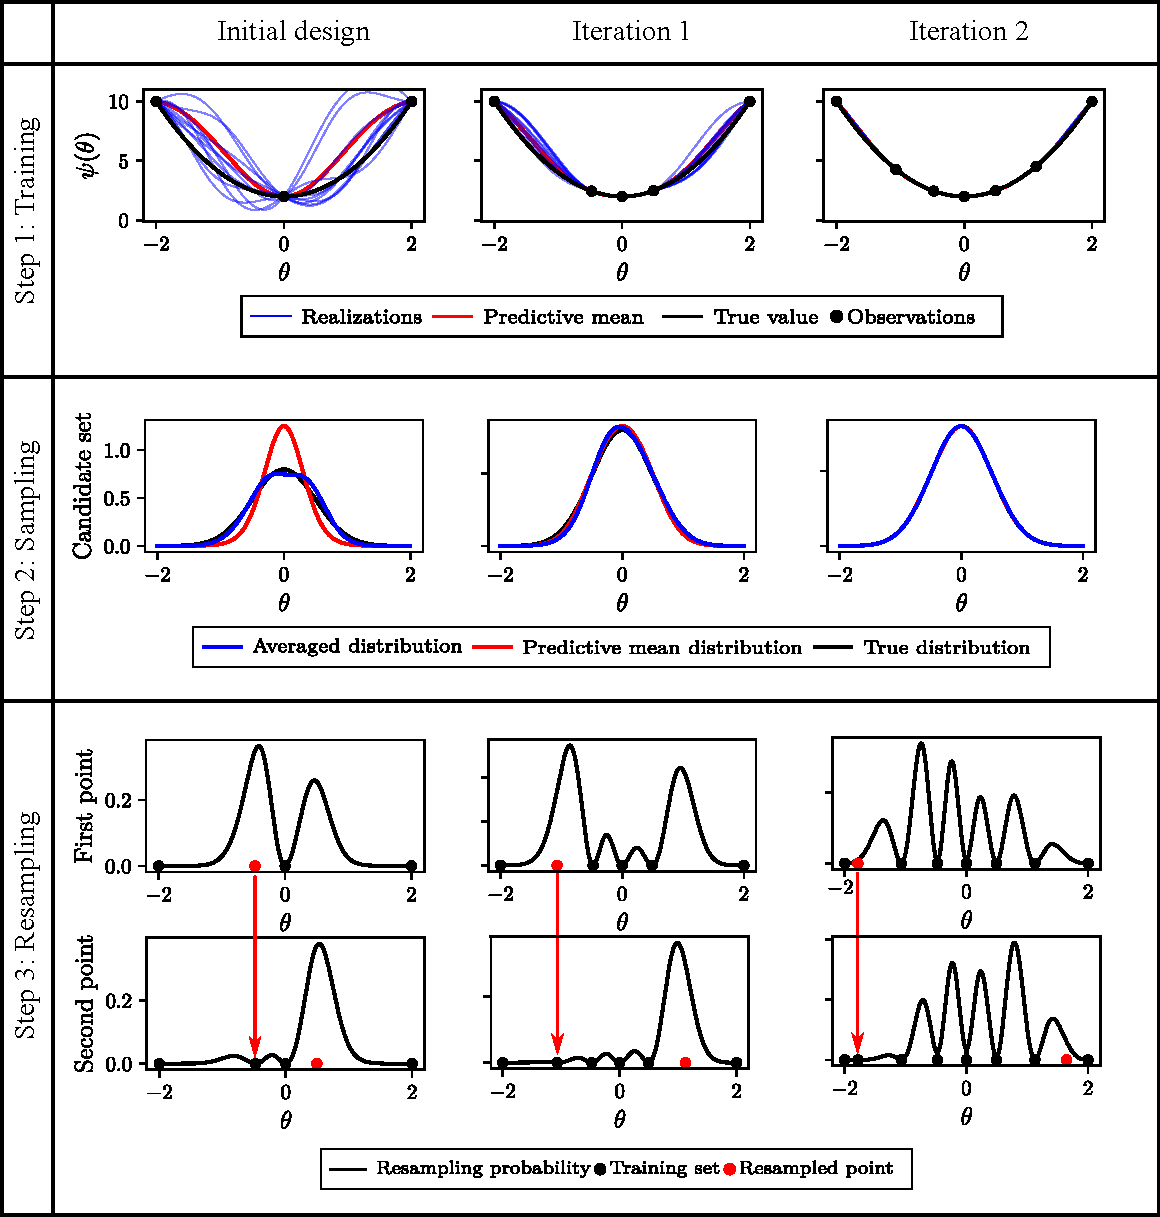
\includegraphics[width=\linewidth]{figures/surr/fig_1.pdf}
  \caption{Illustration of two iterations of the Algorithm~\ref{alg:adapt_surr}. Different columns correspond to different iterations of the algorithm while different rows correspond to different steps of the algorithm. The first row shows the surrogate model of the hyperparameter, $\tilde{\psi}(\theta, \omega)$. The second row shows the candidate set distribution, $\approxp{(k)}{\btheta \mid \yobs}$. The third and fourth rows show the resampling probability distribution for the first and second selected points respectively.}
  \label{fig:surr:fig_1}
\end{figure}

In Fig.~\ref{fig:surr:fig_1} we show the results of the three main steps of two consecutive iterations of Algorithm~\ref{alg:adapt_surr}. Different columns correspond to different iterations while different rows correspond to different steps of the algorithm. In the first row we show the surrogate model of the hyperparameter, $\tilde{\psi}^{(\omega)}(\theta)$, at different iterations. The black line corresponds to the true value, $\psi(\theta)$, while the blue lines correspond to different realizations of the \gls{hgp}. The red line corresponds to the predictive mean of the \gls{hgp}. Due to the simplicity of the problem, only two iterations are sufficient to obtain an excellent approximation of the hyperparameter. Notably, the predictive mean is not a good approximation of the true value at the first iteration, which motivates the need to consider different realizations of the \gls{hgp}.

\smallskip
In the second row we show the candidate set distribution, $\mathrm{p}^{(k)}(\btheta \mid \data)$, at different iterations. The candidate set of points is sampled from this distribution. The black line corresponds to the true distribution, $\propto \exp \phi(\theta, \psi_{\theta})$, while the red line corresponds to the one obtained from the predictive mean, $\propto \exp \phi(\theta, \mathbb{E}_{\omega} \left[ \tilde{\psi}^{(\omega)}(\theta)\right])$. The blue line corresponds to the one obtained by averaging over different realizations of the \gls{hgp}, as done in Eq.~\eqref{eq:avg_dist}. As we can see, at least only where the variance of the \gls{hgp} is large, the averaged distribution is much less peaked than the one obtained from the predictive mean and, therefore, more representative of the actual uncertainty. After the first iterations, the candidate set distribution becomes very close to the true distribution, indicating that the algorithm has converged. 

\smallskip
Finally, the third and fourth rows show the resampling probability distribution for the first and second selected points, respectively. We remind the reader that each point is resampled from the candidate set distribution with resampling weights proportional to the variance of the potential, as discussed in \S\ref{sc:surr:select}. Hence, the resampling probability distribution is the product of the candidate set distribution and the resampling weights. Moreover, after each point is selected, the variance is updated to account for the expected variance improvement, as discussed in \S\ref{sc:surr:select}. In the Figure, the black dots correspond to the training set while the red dots correspond to the randomly resampled points.

\subsection{Test Case 1: Drag of a Sphere}
\label{sc:tc1}

In this section we revisit the test case of the drag of a sphere presented in \S\ref{sc:cmp:test_case}, where an algebraic empirical correlation is used to model the drag coefficient of a sphere as a function of the Reynolds number and 3 parameters. In this context, this test case is particularly interesting because of the availability of a reference solution, which was computed using the exact \gls{cmp} method. The availability of a reference solution allows us to compare the precision of our surrogate-based approaches with the exact \gls{cmp} method.

\smallskip
Moreover, we compare the precision of our adaptive \gls{hgp} sampling strategy with one-shot sampling strategies, such as \gls{lhs}, and with \gls{lpgp} strategies, which build a surrogate model of the potential directly. 

\bigskip
The \glspl{hgp} are all built using \glspl{gp} with constant mean and elliptical \gls{rbf} covariance. Jeffrey's prior is used to regularize the \gls{map} optimization of the covariance strength while a uniform prior is used for the constant mean and the length scales. In all our tests we use a small initial training set of size 5, $\ntrain^{(0)}=5$, fix the number of iterations to $30$ and the number of points to be added to the training set to 10, ${\nresample}=10$. The candidate set is constructed by sampling $400$ points from $20$ different random trajectories of the surrogate models. During each iteration, we measure the relative error on the potential, $\mathcal{E}_{\mathrm{rel}}$, which is defined as:

\begin{equation}
    \left.
        \begin{aligned}
            &\mathcal{E}_{\mathrm{rel}} = \sqrt{\frac{\displaystyle\sum_{\btheta_i \in \boldsymbol{\Theta}_{\mathrm{cmp}}}\mathbb{E}_{\boldsymbol{\omega}}\left[\left(\mathrm{\phi(\btheta \mid \bpsi(\btheta_i))-\mathrm{\phi}(\btheta \mid \tilde{\bpsi}(\btheta_i))}\right)^2\right]}{\displaystyle\sum_{\btheta_i \in \boldsymbol{\Theta}_{\mathrm{cmp}}}\mathrm{\phi(\btheta_i \mid \bpsi(\btheta))}^2}} \;.\\
        \end{aligned}
    \right. 
\label{eq:surr:err}
\end{equation}

The error estimate is computed on 10'000 independent points, the set $\boldsymbol{\Theta}_{\mathrm{cmp}}$, which was separately constructed by sampling the true distribution. Each test is performed $30$ times, starting from a different initial training set design, and the results are averaged.

\begin{figure}[htbp]
    \centering
    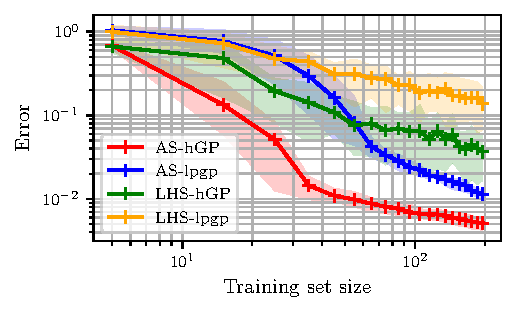
\includegraphics[width=0.7\linewidth]{figures/surr/fig_2.pdf}
    \caption{Relative error on the potential for the 4 different strategies as function of the training set size with $N_0=5$ and ${\nresample}=10$.}
    \label{fig:surr:fig_2}
\end{figure}

Fig.~\ref{fig:surr:fig_2} shows the behavior of the error estimate, computed with Eq.~\eqref{eq:surr:err}, as a function of the training set size for the 4 strategies. 
The two adaptive strategies show a faster convergence rate than the two one-shot strategies. The rapid decrease of the error is due to the fact that iterative strategies focus the computational effort on the regions of the parameter space that are effectively visited a posteriori, while one-shot strategies focus their effort on the entire parameter space. Moreover, iterative strategies are less sensitive to the initial training set design and quickly converge to a good approximation of the posterior distribution, even when the initial training set is small. This is not the case for one-shot strategies, which require many training points to fill the entire parameter space.

\smallskip
Finally, \gls{hgp} strategies are consistently more efficient than their \gls{lpgp} counterparts. The \gls{hgp} strategies model the hyperparameters directly and preserve the structure of the likelihood function while \gls{lpgp} strategies model the potential directly, losing information about the structure of the likelihood function. This is particularly important when the likelihood function is very sensitive to the model parameters, $\btheta$, as it is often the case in calibration problems, and the function $\bpsi(\btheta)$ is easy to learn.

\begin{figure} [htbp]
   \centering
   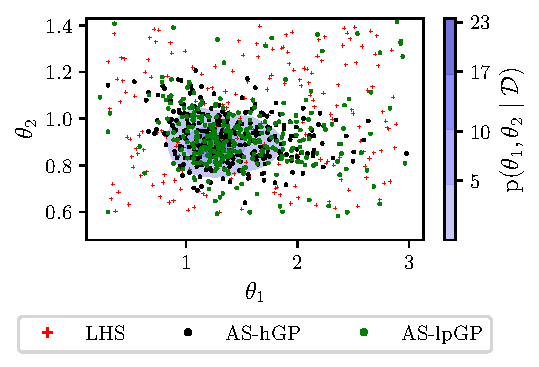
\includegraphics[width=0.7\linewidth]{figures/surr/fig_3.pdf}
      \caption{Training grid design (projected on the first two coordinates). The blue region corresponds to the \gls{kde} of the posterior distribution.}
      \label{fig:surr:fig_3}
\end{figure}

The final training grid design, projected on the first two coordinates, for the different strategies is shown in Fig.~\ref{fig:surr:fig_3}. The \gls{lhs} design is shown in red, while black and green points correspond to the ones of the \gls{as}-\gls{hgp} and \gls{as}-\gls{lpgp} strategies respectively. The blue region corresponds to the \gls{kde} of the joint posterior distribution, which is obtained by sampling 100'000 points from Eq.~\eqref{eq:cmp:cmp}. The picture shows that adaptive strategies are able to place more training points near the mode of the posterior distribution and are hence more efficient in reducing the error on the potential. The training set of the \gls{as}-\gls{hgp} strategy is more concentrated than the one of the \gls{as}-\gls{lpgp} strategy, which is due to the fact that the former models the hyperparameters directly and is therefore able to learn more efficiently the structure of the likelihood function.

\subsection{Test Case 2: Design Under Uncertainty}
\label{sc:tc2}

In this section we illustrate how the \gls{as}-\gls{hgp} strategy can be used to solve a design problem.

\smallskip
A common approach in Computer Aided Design is to use a computational model to predict one or more \glspl{qoi} as functions of a set of design variables. However, as noted in the introduction, such models often depend on unknown parameters that must be calibrated against experimental data. Calibration yields a posterior distribution over the parameters, which can then be propagated to quantify uncertainty in the \glspl{qoi} across the design space. Crucially, reliable uncertainty estimates require explicit treatment of model error, ignoring it leads to overconfident predictions. The design problem therefore consists of finding the set of design variables that maximizes or minimizes a chosen functional of the \glspl{qoi}, while properly accounting for the relevant uncertainties.


\begin{figure}[htbp]
  \centering
  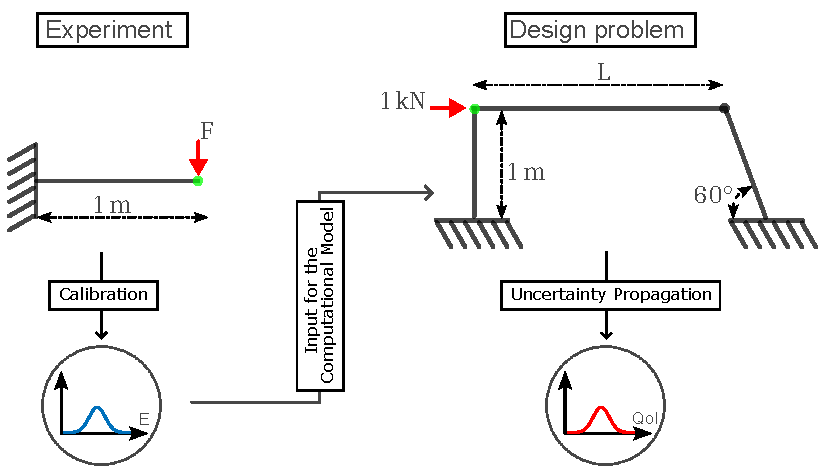
\includegraphics[width=0.9\linewidth]{figures/surr/fig_4.pdf}
  \caption{Schematic representation of a design problem under uncertainty.}
  \label{fig:surr:fig_4}
\end{figure}

In this test case, we consider a simple design problem: estimating the horizontal displacement of a node in a planar frame when a material property is uncertain and must be inferred from observations. The setup is shown schematically in Fig. 4. The design structure (right) consists of a horizontal beam spanning two vertical columns, clamped at the base. The design variable is the beam length $L$, and the response is the horizontal displacement of the top-left node (highlighted in green). The Young’s modulus $E$ is treated as unknown and is calibrated using the experiment in Fig.~\ref{fig:surr:fig_4} (left). After calibration, the posterior distribution of $E$ is propagated through the computational model to solve the design problem, yielding the posterior distribution of the targeted \gls{qoi}. To solve the design problem, we use a computer code which models each beam as an Euler-Bernoulli beam with linear elastic material behavior, a well known approximation in solid mechanics~\cite{eb_beams}.

\subsubsection{Calibration}

\smallskip
The experimental setup does not generally correspond to the design setup. In our case, we assume that the experimental observations correspond to the tip displacement of a single cantilever beam, clamped at one end and loaded at the other end with a variable vertical force, $F$. A total of 10 observations are available for different values of $F$ ranging from $0$ to $1$ kN. For simplicity, we calibrate the product $EI$, where $I = h t^3/12$ is the second moment of area of the beam's cross-section, $h$ and $t$ being the width and thickness of the beam respectively. In order to mimic the effect of model error, we assume that the real system is made of nonlinear material, whose material law is given by,

\begin{equation}
  \left.
      \begin{aligned}
          \ubar{\sigma} &= \dfrac{E(\epsilon_{\mathrm{eq}})}{1-\nu^2} \begin{bmatrix}
            1 & \nu & 0 \\
            \nu & 1 & 0 \\
            0 & 0 & \dfrac{1-\nu}{2}
          \end{bmatrix} \ubar{\epsilon}\;, \\
          E(\epsilon_{\mathrm{eq}}) &= E_1 + (E_2 - E_1) \dfrac{1}{1+\exp(-k(\epsilon_{\mathrm{eq}} - \epsilon_0))}\;.
      \end{aligned}
  \right.
  \label{eq:surr:young}
\end{equation}

Where $\ubar{\sigma}$ and $\ubar{\epsilon}$ are the stress and strain tensors in Voigt notation, $\nu = 0.3$ is the Poisson's ratio. The Young's modulus depends on the equivalent strain, $\epsilon_{\mathrm{eq}}$, and has a bilinear behavior. Specifically, it varies from $E_1 = 210$ GPa to $E_2 = 500$ GPa, with a smooth transition centered at $\epsilon_0 = 10^{-5}$ and with slope $k=10^{6}$. This ensures that the material behaves as a linear elastic material for small strains, with Young's modulus $E_1$, and becomes stiffer as the strain increases, effectively introducing a nonlinearity in the system. The true response of the system is computed using a \gls{fe} model based on Q4 elements and Newton-Raphson iterations to solve the nonlinear problem~\cite{fe_method}.

\begin{figure}[htbp]
  \centering
  \begin{subfigure}{0.49\linewidth}
    \centering
    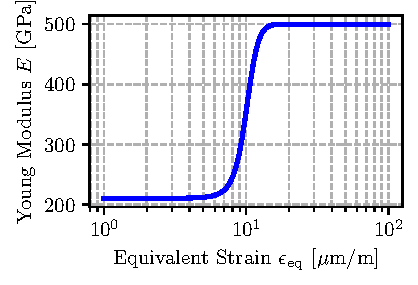
\includegraphics[width=\linewidth]{figures/surr/fig_5a.pdf}
    \caption{Material law.}
  \end{subfigure}\hfill
  \begin{subfigure}{0.49\linewidth}
    \centering
    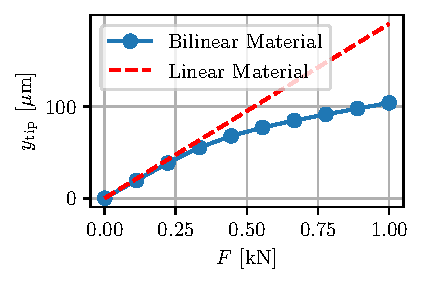
\includegraphics[width=\linewidth]{figures/surr/fig_5b.pdf}
    \caption{Load-displacement curve.}
  \end{subfigure}
  \caption{Bilinear material law and load-displacement curve. For the latter, the linear behavior is the one predicted by the Euler-Bernoulli beam theory with $E = 210$ GPa.}
  \label{fig:surr:fig_5}
\end{figure}

% Make a table containing the geometric and material properties of the beam
\begin{table}
  \centering
  \begin{tabular}{|c|c|c|c|c|c|}
    \hline
    $L$ [m] & $h$ [m] & $t$ [m] & $E_1$ [GPa] & $E_2$ [GPa] & $\nu$ \\ \hline
    1.0        & 0.1     & 0.1      & 210         & 500         & 0.3   \\ \hline
  \end{tabular}
  \caption{Geometric and material properties of the beams.}
  \label{tab:surr:beam}
\end{table}

The material law and the load-displacement curve are shown in Fig.~\ref{fig:surr:fig_5}. The nonlinear behavior of the material introduces a model error when the Euler-Bernoulli beam theory is used to model the system. A centered Gaussian white noise (with standard deviation proportional to $1\%$ of the synthetic observed value) is then added to the output of the FE model in order to mimic the effect of experimental errors. The geometric and material properties of the beams are reported in Tab.~\ref{tab:surr:beam}. The design problem uses the same geometric and material properties, except for the length of the beams, which is reported in Fig.~\ref{fig:surr:fig_4}.

\smallskip
The model error is modeled using a zero mean \gls{gp} with the following covariance function,

\begin{equation}
    k(F, F'; \sigma, l) = \sigma^2 \ FF'\ \exp \left(-\frac{(F-F')^2}{2 l^2}\right) \;.
    \label{eq:cov_beam}
\end{equation}

The covariance function is the product of a \gls{rbf} covariance and a linear covariance. This ensures that the model error is zero when $F=0$, a physical constraint of the system, and that the model error increases as $F$ increases, which is a reasonable assumption since the nonlinearity of the system increases with $F$. As remarked in \cite{hagan_2014}, the choice of the covariance function is crucial to avoid identifiability issues between the model error and the calibration parameters. A uniform prior is used for the hyperparameters of the covariance function, $\sigma$ and $l$, and for the calibration parameter, $EI$.

\smallskip
In this test case, we need to construct 3 \glspl{hgp}, one for each hyperparameter of the covariance function and one for the correction factor. The \glspl{hgp} are built using \glspl{gp} with constant mean and \gls{rbf} covariance. The hyperparameters of the \glspl{hgp} are estimated using \gls{mle}. The initial training set consists of 5 observations and is increased by 1 point for each iteration. Due to the small number of hyperparameters involved and the simplicity of the calibration problem (only a single calibration parameter), a total of 50 iterations proved to be sufficient to reach satisfactory results.

\begin{figure}[htbp]
  \centering
  \begin{subfigure}{0.49\linewidth}
    \centering
    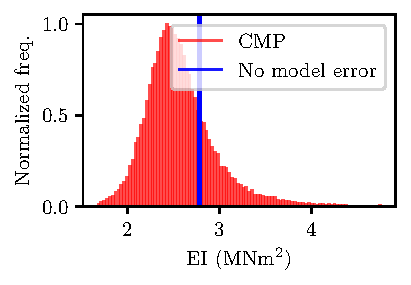
\includegraphics[width=\linewidth]{figures/surr/fig_6a.pdf}
    \caption{Posterior distribution of $EI$.}
  \end{subfigure}\hfill
  \begin{subfigure}{0.49\linewidth}
    \centering
    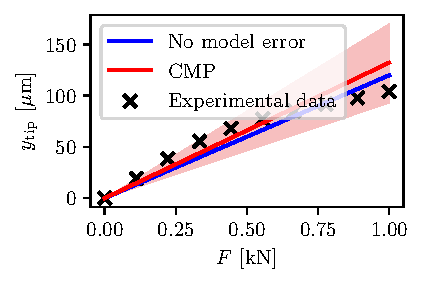
\includegraphics[width=\linewidth]{figures/surr/fig_6b.pdf}
    \caption{Response of the computer model.}
  \end{subfigure}
  \caption{Posterior distribution of the flexural rigidity, $EI$, and response of the computer model. For the latter, solid lines correspond to the mean prediction while shaded areas correspond to the $95\%$ confidence interval.}
  \label{fig:surr:fig_6}
\end{figure}

The posterior distribution of the flexural rigidity, $EI$, and the response of the computer model are shown in Fig.~\ref{fig:surr:fig_6} for both a \gls{cmp} calibration and a calibration without considering the model error term. We note that the posterior distribution of the flexural rigidity is much wider when the model error is considered, which is a direct consequence of the additional uncertainty introduced by the model error. This is a desirable feature of the \gls{cmp} method, which yields a posterior distribution that reflects the fact that no single value of $EI$ can perfectly fit the observations. The larger uncertainty on $EI$ is also reflected in the response of the computer model, which is computed by propagating the uncertainty on $EI$ in the computer model. Not considering the model error leads to an overconfident prediction.

\begin{figure}[htbp]
  \centering
  \begin{subfigure}{0.49\linewidth}
    \centering
    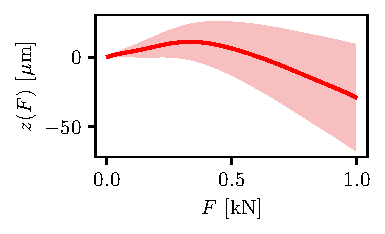
\includegraphics[width=\linewidth]{figures/surr/fig_7a.pdf}
    \caption{Model error as a function of the tip load, $F$.}
  \end{subfigure}\hfill
  \begin{subfigure}{0.49\linewidth}
    \centering
    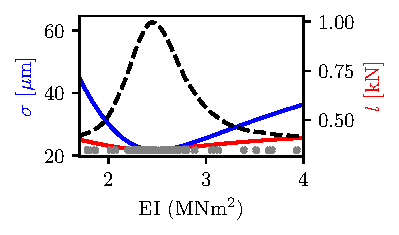
\includegraphics[width=\linewidth]{figures/surr/fig_7b.pdf}
    \caption{\gls{cmp} hyperparameters as a function of $EI$.}
  \end{subfigure}
  \caption{On the left, the model error as a function of the tip load, $F$. The solid line corresponds to the predictive mean, while the shaded area corresponds to the $95\%$ confidence interval. On the right, the \gls{cmp} hyperparameters as a function of $EI$ (covariance strength in blue and length scale in red). The dashed lines correspond to a visual representation of the posterior distribution of $EI$ and the gray dots correspond to the final \gls{hgp} training set.}
  \label{fig:surr:fig_7}
\end{figure}

In Fig.~\ref{fig:surr:fig_7} we show the model error as a function of the tip load, $F$, and the \gls{cmp} hyperparameters as a function of $EI$. As we can see, the model error goes to zero when $F=0$ and increases as $F$ increases, as expected. The \gls{cmp} hyperparameters depend on the calibration parameter, $EI$, and the \glspl{hgp} are able to learn this dependence efficiently. The training set of the \glspl{hgp} is concentrated in the region of high posterior probability, which is a desirable feature of the \gls{as}-\gls{hgp} strategy.

\subsubsection{Design Problem}

\begin{figure}[htbp]
  \centering
  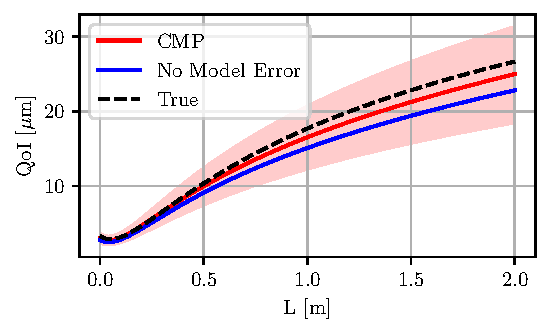
\includegraphics[width=0.7\linewidth]{figures/surr/fig_8.pdf}
  \caption{Horizontal displacement of the top left node of the flat frame as a function of the length of the horizontal beam, $L$. Solid lines correspond to the mean prediction while shaded areas correspond to the $95\%$ confidence interval.}
  \label{fig:surr:fig_8}
\end{figure}

Finally, the \gls{qoi}, namely horizontal displacement of the top left node of the flat frame as a function of the length of the horizontal beam, $L$, the design variable, is shown in Fig.~\ref{fig:surr:fig_8}. The prediction is obtained by propagating the uncertainty on $EI$ to the \gls{qoi} in the computer model. In this case, the mean prediction computed by propagating the \gls{cmp} posterior distribution is very close to the true one, which is computed by using the nonlinear material law. Most importantly, though, the \gls{cmp} confidence interval contains the true value of the \gls{qoi} for all values of $L$, which is a direct consequence of properly accounting for the model error in the calibration process. This is not the case when the model error is not considered, which leads to an overconfident prediction whose confidence interval does not contain the true value of the \gls{qoi}.

\smallskip
Overall, this test case underlines the importance of properly accounting for the model error in the calibration process to obtain reliable predictions and showcases how the \gls{as}-\gls{hgp} strategy can be used to solve design problems under uncertainty.

\section{Conclusion}
\label{sc:conclusion}

In this chapter we have presented a surrogate-based approach to accelerate the \gls{cmp} calibration framework. The \gls{cmp} method consists of a modular framework that separates the estimation of the model error hyperparameters $\bpsi$ from the estimation of the calibration parameters $\btheta$. This estimation relies on an implicit definition of a mapping $\psimap : \btheta \mapsto \bpsi$ that is defined as the solution of an optimization problem. This implicit definition of the mapping $\psimap$ is a key feature of the \gls{cmp} method, which allows it to be very flexible and applicable to a wide range of problems. However, it also makes the estimation of the mapping $\psimap$ computationally expensive since it requires solving an optimization problem for each value of $\btheta$. To mitigate this problem, we have proposed to build a surrogate model for the mapping $\psimap$ using \glspl{gp}, which we call \glspl{hgp}. The surrogate model for the mapping $\psimap$ allows us to efficiently estimate the potential, $\phi(\btheta \mid \psimap)$, and therefore the posterior distribution of the calibration parameters, $\mathrm{p}(\btheta \mid \data)$. We have also proposed an \gls{as} strategy to iteratively improve the surrogate model for the mapping $\psimap$ by adding new training points that are selected based on their expected improvement on the surrogate model. Finally, we have presented a simplified version of the proposed method that builds a surrogate model for the potential directly, which we call \gls{lpgp}.

\smallskip
In the vast majority of cases, the bulk of the computational cost of any calibration method is due to evaluation of the forward model. The \gls{cmp} method, by reducing the dimensionality of the calibration problem, requires fewer evaluations of the forward model than traditional calibration methods, but does not eliminate the need for such evaluations. Furthermore, we did not include the construction of a surrogate model for the forward model in the proposed online strategies.

\smallskip
While considering the forward model $f(\bx;\btheta)$ as an extra hyperparameter of the \gls{cmp} method and building a surrogate model for it is a promising direction to further reduce the computational cost of the \gls{cmp} method, it is not straightforward to do so. Indeed, this would require coupling the calibration software and hardware with the forward model software and hardware, which can be a non-trivial task. Moreover, the surrogate model for the forward model generally has different requirements than the surrogate model for the mapping $\psimap$. For instance, the surrogate model for the forward model needs to be used for different tasks such as optimization, uncertainty propagation, etc., while the surrogate model for the mapping $\psimap$ is only used to estimate the potential and the posterior distribution of the calibration parameters. 

\smallskip
For all the reasons above, we decided to focus on building a surrogate model just for $\psimap$, thus creating a modular framework that can be used to perform calibration in a reduced dimensional space at a reduced computational cost. 

\smallskip
In the next chapter we will present an application of the calibration frameworks discussed in the first part of this thesis to a real-world problem, namely the calibration of a complex \gls{cfd} model of high-enthalpy hypersonic jet.